\documentclass{standalone}
\usepackage{tikz}
\usetikzlibrary{arrows}
\begin{document}
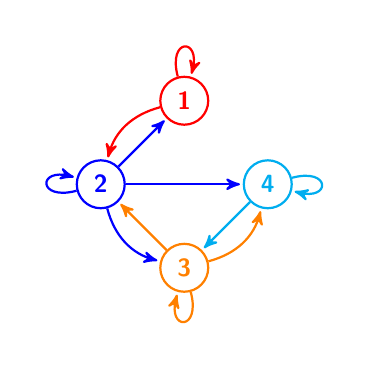
\begin{tikzpicture}[->,>=stealth',shorten >=1pt,auto,node distance=1.5cm,
    thick,main node/.style={circle,draw,font=\sffamily\small\bfseries}]

\node[main node, color=red] (1) {1};
\node[main node, color=blue] (2) [below left of=1] {2};
\node[main node, color=orange] (3) [below right of=2] {3};
\node[main node, color=cyan] (4) [below right of=1] {4};

\path[every node/.style={font=\sffamily\small}]
(1) edge [bend right, draw=red] node[left] {} (2)
    edge [loop above, draw=red] node {} (1)
(2) edge [draw=blue] node [right] {} (1)
    edge [draw=blue] node {} (4)
    edge [loop left, draw=blue] node {} (2)
    edge [bend right, draw=blue] node[left] {} (3)
(3) edge [draw=orange] node [right] {} (2)
    edge [bend right, draw=orange] node[right] {} (4)
    edge [loop below, draw=orange] node {} (3)
(4) edge [draw=cyan] node [left] {} (3)
    edge [loop right, draw=cyan] node {} (4);
\end{tikzpicture}
\end{document}